\section{Global System View}

The proposed system consists of a GUI that will be on a laptop and up to 5 7.5cm spheres.  Figure~\ref{fig:GSV1} shows an idea of how experiments will be conducted by researchers using this system.  As it shows, they will have a laptop with the necessary hardware and software on a jet ski and at least one sphere to throw into the water.

\begin{figure}[H]
	\centering
	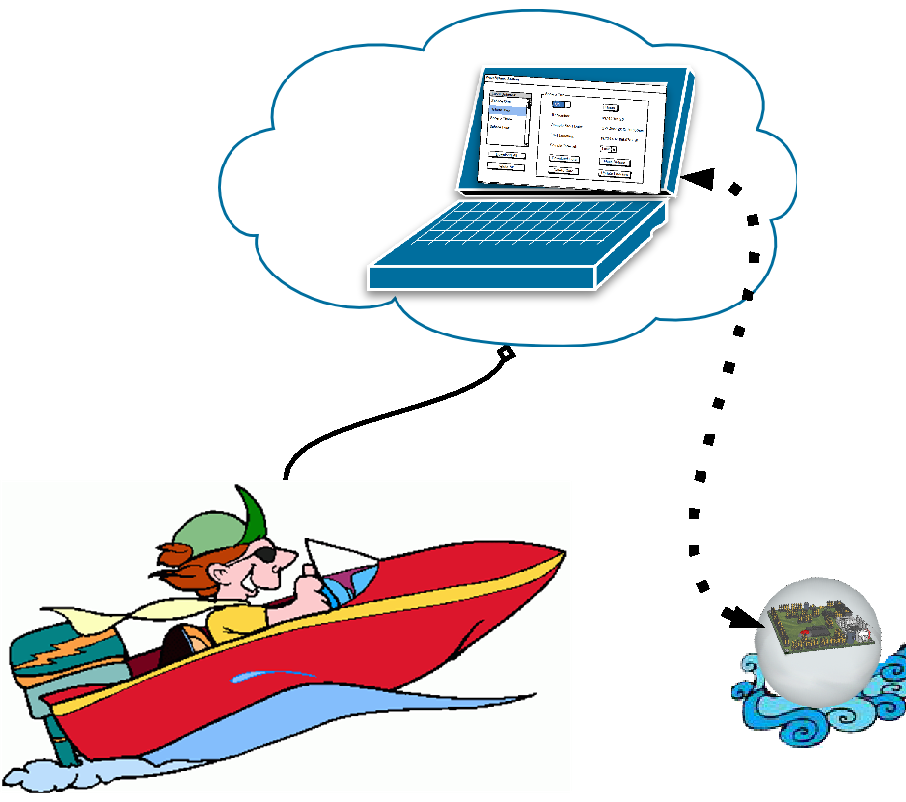
\includegraphics[scale=0.5]{img/GSV1}
	\caption{A rough model of the interaction between the base and one sphere. \label{fig:GSV1}}
\end{figure}

The previous figure shows the interaction within the computer and one sphere, which is the scope of this project, but the base will be able to handle more than one.  Figure~\ref{fig:GSV2} shows how the interaction would be between multiple spheres, in this case 4, and the base station (laptop).

\begin{figure}[H]
	\centering
	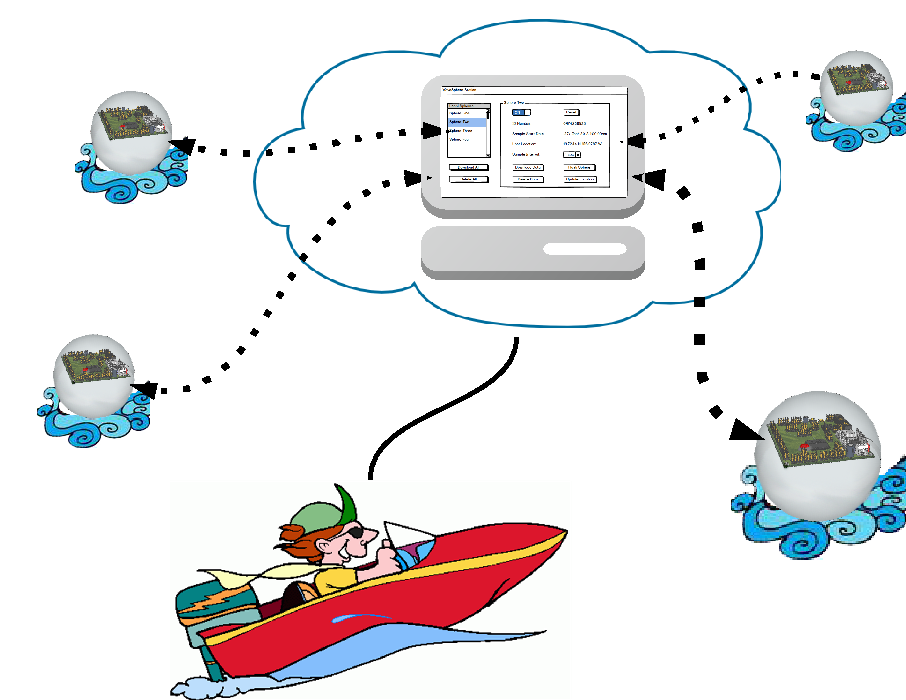
\includegraphics[scale=0.6]{img/GSV2}
	\caption{A rough model of the interaction between the base and multiple spheres. \label{fig:GSV2}}
\end{figure}

Figure~\ref{fig:GSV3} gives a closer look to the interaction between spheres and the base station software.  It shows a software prototype that will be in charge of controlling the necessary hardware in order to communicate with the spheres and perform the necessary tasks such as transfer data from spheres, locate a sphere, reset a sphere or turn off a sphere.  Note that this is a GUI prototype and might be missing some functionality that will form part of this project final system software.  

\begin{figure}[H]
	\centering
	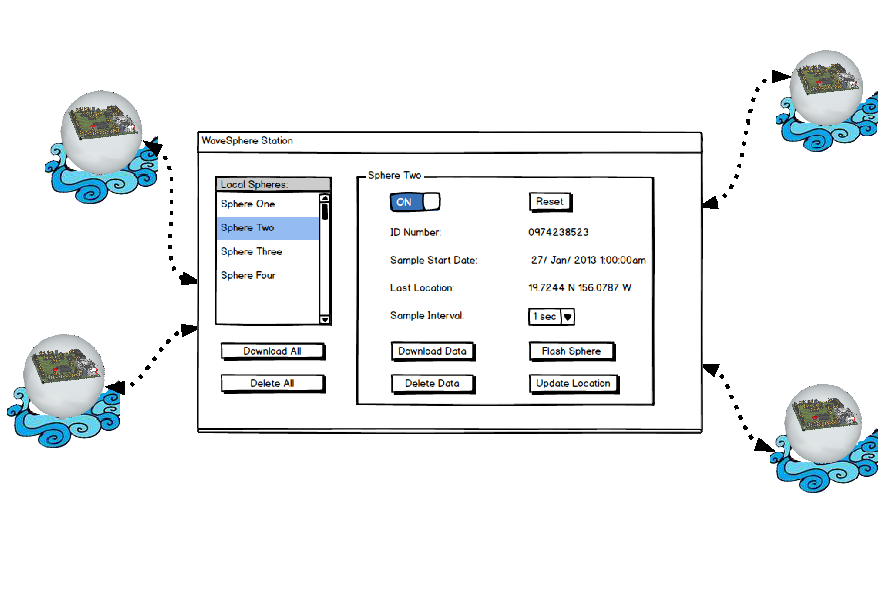
\includegraphics[scale=0.6]{img/GSV3}
	\caption{A closer look to the interaction between the base and the spheres. \label{fig:GSV3}}
\end{figure}

Finally, figure~\ref{fig:sphere} shows an idea on how the sphere will look like.  A PCB board containing all the necessary hardware will be located axisymmetrically inside the sphere.  This board will be adhered to the sphere such that the hardware does not move freely inside the sphere during the experiments.

\begin{figure}[H]
	\centering
	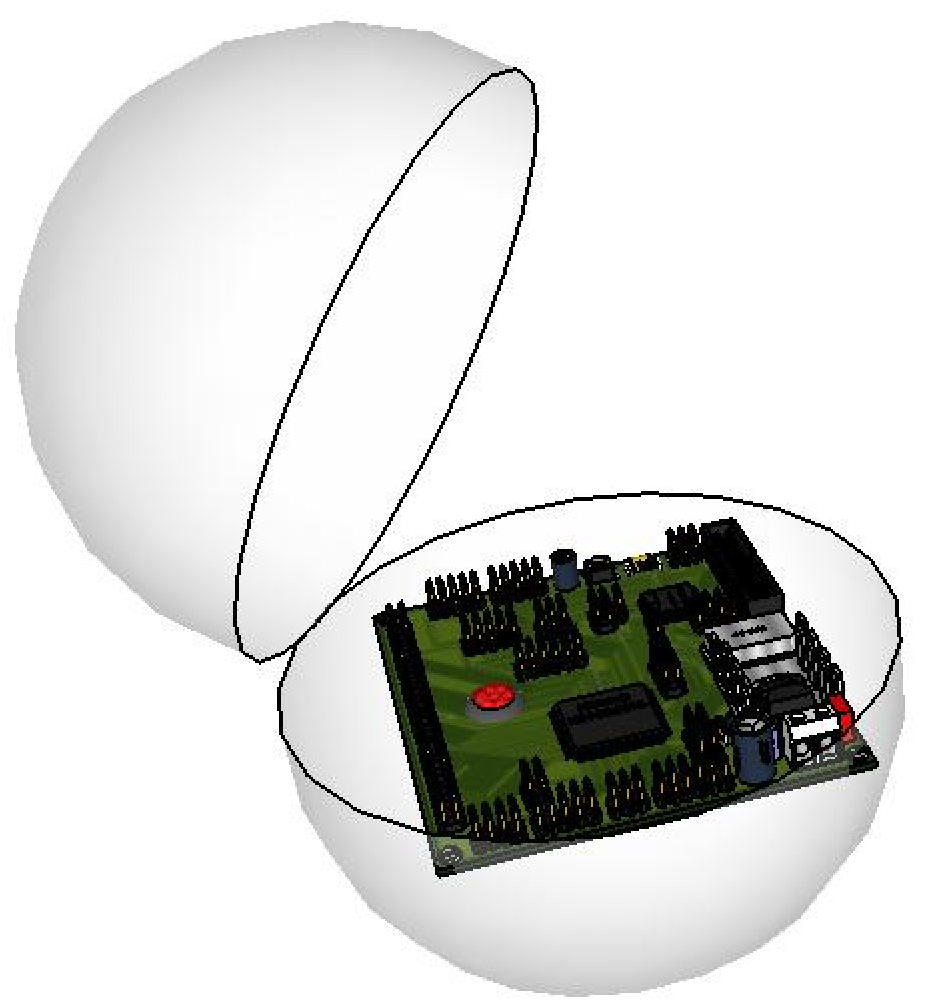
\includegraphics[scale=0.6]{img/Sphere_001}
	\caption{Rough model of hardware inside the sphere. \label{fig:sphere}}
\end{figure}